%!TEX TS-program = xelatex
%!TEX encoding = UTF-8

% 使用自定义的文档类 AJbook.cls. 自动载入 xeCJK. 需要额外档案如下:
% font-setup-open.tex, coverpage.tex, titles-setup.tex, mycommand.sty, myarrows.sty
% 文档类选项 (key/val 格式):
% draftmark = true (未定稿, 底部显示日期) 或 false (成品), 默认 false,
% colors = true (链接带颜色无框) 或 false (黑色无框), 默认 true,
% traditional = true (繁体中文) 或 false (简体中文), 默认 false,
% coverpage = 封面档档名, 默认为空 (此时不制作封面), 一般是 .tex 档, 若为 *.pdf 的形式则直接引入 PDF 页面.
% fontsetup = 字体设置档档名,
% titlesetup = 章节格式设置档名.

% 注意: 如果文中未使用 \cite 和 \index 命令, 则可能报错.

% 需动用 imakeidx + xindy (两份索引), biblatex + biber (书目). 
% 索引用土法进行中文排序: 如 \index{zhongwen@中文} 等.
\PassOptionsToPackage{quiet}{fontspec}	% 避免 CJK 字体警告
\documentclass[
	draftmark = true,   % 草稿模式下, 每页底部将打印相关版本信息.
%	traditional = true,
%	colors = false,
	coverpage = cover.pdf,
    geometry = a4,    % 版面设置, 目前仅容许 a4, b5, 默认 b5, 其它字串则不作自动设置.
	fontsetup = font-setup-open.tex,
	titlesetup = titles-setup.tex
]{AJbook}

\usepackage{bm}  % 数学粗体
\usepackage{mathrsfs}
\usepackage{stmaryrd} \SetSymbolFont{stmry}{bold}{U}{stmry}{m}{n}	% 避免警告 (stmryd 不含粗体故)
\usepackage{array}
\usepackage{makecell}	% 便于制表
\usepackage{tikz-cd}  % 使用 TikZ 绘图
\usetikzlibrary{positioning, patterns, calc, matrix, shapes.arrows, shapes.symbols}
\usetikzlibrary{decorations.pathreplacing,calligraphy}
\usepackage{braids}
\usepackage{tqft}
\usepackage{ytableau}
\usepackage{multirow}
\usepackage{threeparttable}	% 表格注释
\usepackage[inkscapearea=page]{svg}	% 插入 svg 图形
\graphicspath{{imgs/}}	% 设定图片目录
\usepackage{pythonhighlight}
\usepackage{subfigure} % 并排图片宏包


\usepackage{annotate-equations} % 为公式添加注释
\renewcommand{\eqnannotationfont}{\ttfamily\footnotesize}  % 注释文本字体,替换为等宽字体
\tikzset{annotate equations/text/.style={font=\eqnannotationfont,color=WildStrawberry}}  % 注释文本样式,红色

% 定义颜色
\usepackage{xcolor}
\definecolor{yellow}{HTML}{b58900}
\definecolor{orange}{HTML}{cb4b16}
\definecolor{red}{HTML}{dc322f}
\definecolor{magenta}{HTML}{d33682}
\definecolor{violet}{HTML}{6c71c4}
\definecolor{blue}{HTML}{268bd2}
\definecolor{cyan}{HTML}{2aa198}
\definecolor{green}{HTML}{859900}
\definecolor{base03}{HTML}{002b36}
\definecolor{base02}{HTML}{073642}
\definecolor{base01}{HTML}{586e75}
\definecolor{base00}{HTML}{657b83}
\definecolor{base0}{HTML}{839496}
\definecolor{base1}{HTML}{93a1a1}
\definecolor{base2}{HTML}{eee8d5}
\definecolor{base3}{HTML}{fdf6e3}
\definecolor{LemonChiffon}{HTML}{fffacd}  % 柠檬绸色
\definecolor{Teal}{HTML}{008080}  % 青色
\definecolor{Olive}{HTML}{808000}  % 橄榄色

% PGF plots 用于封面绘制
\usepackage{pgfplots}
\pgfplotsset{compat=newest}

% 可以修改章节编号的深度
% \setcounter{secnumdepth}{3}

% 必要时仅引入部分档案
% \includeonly{}

% 生成索引: 选用 xindy + imakeidx
\usepackage[xindy, splitindex]{imakeidx}
\makeindex[
	columns=2,
	program=truexindy,
	intoc=true,
	options=-M texindy -I xelatex -C utf8,
	title={Keyword Index}]	% 名词索引

\usepackage[unicode, bookmarksnumbered]{hyperref}	% 启动超链接和 PDF 文档信息所需
% 设置 PDF 文件信息
\hypersetup{
	pdfauthor = {Imiloin},
	pdftitle = {AJbook 文档类模板},
	pdfkeywords = {Template},
	CJKbookmarks = true}

% 增加表格高度
\renewcommand*\arraystretch{1.5}

% 自订公式的编号 (非必要)
\numberwithin{equation}{section}
\renewcommand{\theequation}{\thesection--\arabic{equation}}

% 自订 figure 的编号 (非必要)
%\numberwithin{figure}{section}
%\renewcommand{\thefigure}{\thechapter--\arabic{figure}}

% 自订 table 的编号 (非必要)
%\numberwithin{table}{section}
%\renewcommand{\thetable}{\thechapter--\arabic{table}}

% 用 bibLaTeX 生成参考文献
% 载入书目库: 文档类业已引入 biblatex + biber
\usepackage[backend=biber]{biblatex}
\addbibresource{references.bib}

\begin{document}
	\frontmatter	% 制作封面和目录.
	% 注意: 为了简化, 本模板不含封面. 请通过文档类的参数进行设置.
	
	\mainmatter		% 正文开始:逐章引入 TeX 代码

	\chapter*{Introduction}
	本文档为 \nolinkurl{Deeplearning.ai} 开设的深度学习系列课程的个人笔记。

	\vspace{1em}
	\begin{flushright}\begin{minipage}{0.2 \textwidth}
		\begin{tabular}{c}
			{By Imiloin} \\
			\href{https://github.com/Imiloin}{Github profile}\\
		\end{tabular}
	\end{minipage}\end{flushright}

	% % % % % % % % % %
	\part{Course Notes}

	\chapter{Neural Networks and Deep Learning}

%%%%
\section{Introduction to Deep Learning}
机器学习本质上就是训练模型来完成\textbf{从输入到输出($\bm{X\to Y}$)的映射}。例如, 给定一张猫的照片, 机器学习模型可以输出``这是一只猫''的结论。

\vspace{0.5\baselineskip} % 半行距

深度学习有3大要点:
\begin{itemize}	
	\item Data
	\item Computation
	\item Algorithms
\end{itemize}

Data可以分为Structured Data和Unstructured Data。Structured Data是指有固定格式的数据, 例如表格、数据库等。Unstructured Data是指没有固定格式的数据, 例如图片、音频、视频等。

Computation是指计算机的计算能力, 例如CPU、GPU、TPU等。

Algorithms是指算法, 例如Logistic Regression、SVM、Neural Networks等。

%%%%
\section{Neural Networks Basics}

表 \ref{tab:notations} 是本章用到的符号说明。为方便起见,所有的向量符号不会加粗,用小写字母表示;同时也不对偏导数进行专门的区分,仍使用$\mathrm{d}$符号表示偏微分。

\begin{table}[ht]
	\centering
	\begin{threeparttable}
	%%
	\caption{Notations}
	%
	\begin{tabular}{clcc}
		\hline
									& \textbf{Notation}                                     & \textbf{Description} & \textbf{Meaning}                                                   \\ \hline
		\multirow{5}{*}{Sizes}      & $m$                                                   & value                & 样本容量                                                               \\
									& $n_x$ / $n_h^{[0]}$                                   & value                & 单个样本的特征数(输入层节点数)                                         \\
									& $n_y$ / $n_h^{[L]}$                                   & value                & 单个样本的标签数(输出层节点数)                                      \\
									& $n_h^{[l]}$ / $n^{[l]}$                               & value                & 第$l$层的神经元个数(隐藏层节点数)                                   \\
									& $L$                                                   & value                & 神经网络的层数                                                         \\ \hline
		\multirow{11}{*}{Objects}   & $x^{(i)} \in \mathbb{R}^{n_x}$                        & vector               & 第$i$个样本数据                                                          \\
									& $X / A^{[0]} \in {\mathbb{R}^{n_x \times m}}$         & matrix               & 输入矩阵                                                               \\
									& $a^{[l](i)} \in \mathbb{R}^{n^{l}}$                   & vector               & 第$i$个样本在第$l$层节点的输出                                                  \\
									& $a_j^{[l]} \in \mathbb{R}^{1 \times {m}}$             & vector               & 第$l$层第$j$个节点的输出                                                         \\
									& $A^{[l]} \in \mathbb{R}^{n^{[l]} \times {m}}$         & matrix               & 第$l$层节点的输出矩阵                                                         \\
									& $y^{(i)} \in \mathbb{R}^{n_y}$                        & vector               & 第$i$个样本的标签                                                         \\
									& $Y \in {\mathbb{R}^{n_y \times m}}$                   & matrix               & 样本标签矩阵                                                           \\									
									& $\hat{y}^{(i)} \in \mathbb{R}^{n_y}$                  & vector               & 第$i$个样本的标签预测值向量                                                \\
									& $\hat{Y} / A^{[L]} \in {\mathbb{R}^{n_y \times m}}$   & matrix               & 标签预测值矩阵($n_y=1$时退化为行向量$\hat{y}$)   						\\
									& $W^{[l]} \in \mathbb{R}^{n^{[l]} \times n^{[l-1]}}$   & matrix               & 第$l$层的权重矩阵                                                               \\
									& $b^{[l]} \in \mathbb{R}^{n^{[l]}}$                    & vector               & 第$l$层的标签偏置值向量                                                        \\\hline
		\multirow{5}{*}{Other}      & $g^{[l]}(z)$                                          & function             & 第$l$层的激活函数                                                         \\
									& $L^{(i)}(\hat{y}^{(i)}, y^{(i)})$                     & function             & 第$i$个样本的代价函数                                                         \\
									& $J(X,W,b,Y)$ or $J(\hat{Y},Y)$                        & function             & 代价函数                                                                        \\
									& $\alpha$								                & value                & 学习率                                                                        \\
									& $\mathrm{d}\mathrm{var}$                              & differential         & 代价函数对变量$\mathrm{var}$的偏微分,即${\partial J}/{\partial \mathrm{var}}$ \\ \hline
	\end{tabular}
	%
	\label{tab:notations} %
	\begin{tablenotes}
		\item[*] 通常情况下$(i)$表示第$i$个样本,而$[l]$表示第$l$层。
	\end{tablenotes}
	%%
	\end{threeparttable}
\end{table}

%%%
\subsection{Binary Classification}
\textbf{二元分类模型}的输入是一个样本$x^{(i)} \in \mathbb{R}^{n_x}$,输出是一个标签$y^{(i)} \in \{0, 1\}$,即$y^{(i)}$只能取0或1且$n_y=1$,对每一个样本得出是或否的结论。

%%%
\subsection{Logistic Regression}
\index{Logistic Regression}

在本节中,由于只考虑一个单层单节点的神经网络,因此省略上标$[l]$,使用简化后的符号如表 \ref{tab:notations_LR} 所示。

\begin{table}[ht]
	\centering
	\begin{threeparttable}
	\caption{Notations in Logistic Regression}
	\begin{tabular}{clcc}
		\hline
									& \textbf{Notation}                         & \textbf{Description} & \textbf{Meaning}                                                   \\ \hline
		\multirow{2}{*}{Sizes}      & $m$                                       & value                & 样本容量                                                               \\
									& $n_x$                                     & value                & 单个样本的特征数(输入层节点数)                                         \\ \hline
		\multirow{8}{*}{Objects}    & $x^{(i)} \in \mathbb{R}^{n_x}$            & vector               & 第$i$个样本数据                                                          \\
									& $X \in {\mathbb{R}^{n_x \times m}}$       & matrix               & 输入矩阵                                                               \\
									& $a^{(i)} / y^{(i)}$                       & binary               & 第$i$个样本的标签实际值                                                        \\
									& $y \in \mathbb{R}^{m}$					& vector               & 标签实际值向量                                                          \\
									& $\hat{y}^{(i)}$                           & binary               & 第$i$个样本的标签预测值                                                  \\
									& $\hat{y} \in {\mathbb{R}^{m}}$            & vector               & 标签预测值向量   					                                     \\
									& $w \in \mathbb{R}^{n_x}$                  & vector               & 权重向量                                                                \\
									& $b$                                       & value                & 标签偏置值                                                            \\ \hline
		\multirow{2}{*}{Other}      & $J(x,w,b,y)$ or $J(\hat{y},y)$            & function             & 代价函数                                                               \\
									& $\mathrm{d}\mathrm{var}$                  & differential         & 代价函数对变量$\mathrm{var}$的偏微分                                    \\ \hline
	\end{tabular}
	\label{tab:notations_LR}
	\end{threeparttable}
\end{table}

对于二元分类模型,相关公式如下:
\begin{equation}
	\hat{y}^{(i)} = \sigma(w^\mathrm{T} x^{(i)} + b) \label{eq:logistic}
\end{equation}
其中sigmoid函数$\sigma(z)$定义为:
\begin{equation}
	\sigma(z) = \frac{1}{1 + \mathrm{e}^{-z}} \label{eq:sigmoid}
\end{equation}
该函数可以把实数域$\mathbb{R}$映射到区间$(0, 1)$,可作为激活函数使用,如图 \ref{fig:sigmoid} 所示。而$z = w^\mathrm{T} x + b$为线性函数,$w$为权重(weight),$b$为偏置(bias)。
\begin{figure}[h!b]
	\centering
	\includesvg[width=8cm]{sigmoid}
	\caption{Sigmoid 函数,关于点(0, 0.5)对称}
	\label{fig:sigmoid}
\end{figure}

\vspace{0.5\baselineskip}
对某一个样本而言,Loss function(误差函数)定义为:
\begin{equation}
	L(\hat{y}^{(i)}, y^{(i)}) = -\left[y^{(i)} \log \hat{y}^{(i)} + (1 - y^{(i)}) \log (1 - \hat{y}^{(i)})\right] \label{eq:loss}
\end{equation}
该函数与方差类似,当样本的误差越大,Loss function的值越大,如图 \ref{fig:loss} 所示。
\begin{figure}[h!b]
	\centering
	\includesvg[width=8cm]{LossFunction}
	\caption{Loss Function 误差函数}
	\label{fig:loss}
\end{figure}

对整个模型而言,Cost function(代价函数)定义为:
\begin{equation}
	J(w, b) = \frac{1}{m} \sum_{i=1}^{m} L(\hat{y}^{(i)}, y^{(i)}) = -\frac{1}{m} \sum_{i=1}^{m} \left[y^{(i)} \log \hat{y}^{(i)} + (1 - y^{(i)}) \log (1 - \hat{y}^{(i)})\right] \label{eq:cost}
\end{equation}
相当于误差函数的平均值。

%%%
\subsection{Gradient Descent}
\index{Gradient Descent}

训练过程使用\textbf{梯度下降(Gradient Descent)算法},即:
\begin{equation}
	\mathrm{var} = \mathrm{var} - \alpha \frac{\mathrm{d}J}{\mathrm{d}\mathrm{var}} \label{eq:gradient}
\end{equation}

其中$\mathrm{var}$为一个需要调整的参数,$\alpha$为学习率(Learning Rate)。对于Logistic Regression,梯度下降算法的表达式为:
\begin{equation}
	\begin{aligned}
	w &:= w - \alpha \frac{\mathrm{d}J}{\mathrm{d}w} \\
	b &:= b - \alpha \frac{\mathrm{d}J}{\mathrm{d}b}
	\end{aligned} 
	\label{eq:gradient_logistic}
\end{equation}
其中$:=$表示赋值,通过不断更新$w$, $b$的值使$J$尽可能小。下面介绍具体实现

\vspace{0.5\baselineskip}
对于一个样本,有
\begin{equation}
	\begin{aligned}
	z &= w^\mathrm{T} x^{(i)} + b \\
	\hat{y}^{(i)} &= \sigma(z) \\
	L(\hat{y}^{(i)}, y^{(i)}) &= -\left[y^{(i)} \log \hat{y}^{(i)} + (1 - y^{(i)}) \log (1 - \hat{y}^{(i)})\right]
	\end{aligned} 
	\label{eq:gradient_logistic_sample}
\end{equation}
进行求导($x$, $y$均为常量),有
\begin{equation}
	\begin{aligned}
	&\frac{\mathrm{d}L}{\mathrm{d}\hat{y}^{(i)}} = -\frac{y^{(i)}}{\hat{y}^{(i)}} + \frac{1 - y^{(i)}}{1 - \hat{y}^{(i)}} \\
	&\frac{\mathrm{d}\hat{y}^{(i)}}{\mathrm{d}z} = \frac{\mathrm{e}^{-z}}{(1 + \mathrm{e}^{-z})^2} = \frac{1}{1 + \mathrm{e}^{-z}}(1 - \frac{1}{1 + \mathrm{e}^{-z}}) = \hat{y}^{(i)}(1 - \hat{y}^{(i)})\\
	\end{aligned}
\end{equation}
用链式法则,有
\begin{equation}
	\frac{\mathrm{d}L}{\mathrm{d}z} = \frac{\mathrm{d}L}{\mathrm{d}\hat{y}^{(i)}} \frac{\mathrm{d}\hat{y}^{(i)}}{\mathrm{d}z} = (-\frac{y^{(i)}}{\hat{y}^{(i)}} + \frac{1 - y^{(i)}}{1 - \hat{y}^{(i)}})\hat{y}^{(i)}(1 - \hat{y}^{(i)}) = \hat{y}^{(i)} - y^{(i)}
\end{equation}
进而有
\begin{equation}
	\begin{aligned}
	\frac{\mathrm{d}L}{\mathrm{d}w_j} &= \frac{\mathrm{d}L}{\mathrm{d}z} \frac{\mathrm{d}z}{\mathrm{d}w_j} = x_j^{(i)} (\hat{y}^{(i)} - y^{(i)}) \quad (1 \leqslant j \leqslant n_x) \\
	\frac{\mathrm{d}L}{\mathrm{d}b} &= \frac{\mathrm{d}L}{\mathrm{d}z} \frac{\mathrm{d}z}{\mathrm{d}b} = \hat{y}^{(i)} - y^{(i)}
	\end{aligned}
\end{equation}

\vspace{0.5\baselineskip}
对于整个训练集,在一个循环中我们对每一个样本都进行一次梯度下降,并对所有样本的梯度进行平均,有
\begin{equation}
	\begin{aligned}
		\frac{\mathrm{d}J}{\mathrm{d}w_j} &= \frac{1}{m} \sum_{i=1}^{m} \frac{\mathrm{d}L}{\mathrm{d}w_j} = \frac{1}{m} \sum_{i=1}^{m} x_j^{(i)} (\hat{y}^{(i)} - y^{(i)}) \quad (1 \leqslant j \leqslant n_x)\\
		\frac{\mathrm{d}J}{\mathrm{d}b} &= \frac{1}{m} \sum_{i=1}^{m} \frac{\mathrm{d}L}{\mathrm{d}b} = \frac{1}{m} \sum_{i=1}^{m} (\hat{y}^{(i)} - y^{(i)})
	\end{aligned}
\end{equation}
得到梯度的平均值后,再进行参数更新,即
\begin{equation}
	\begin{aligned}
	w_j &:= w_j - \alpha \frac{\mathrm{d}J}{\mathrm{d}w} \quad (1 \leqslant j \leqslant n_x) \\
	b &:= b - \alpha \frac{\mathrm{d}J}{\mathrm{d}b}
	\end{aligned} 
\end{equation}
这样就完成了一轮梯度下降的循环。重复多次梯度下降,直到$J$收敛或达到最大迭代次数,就得到了最终的$w$, $b$。

%%%
\subsection{Vectorization}

一个重要的原则是,在训练过程中要避免使用循环,而是使用向量化的方法。向量化可以调用并行计算,相对于循环的串行计算效率更高。\\
要完成下面的矩阵操作,
\begin{equation}
	Z =
	\begin{bmatrix}
		z^{(1)} & z^{(2)} & \cdots & z^{(m)}
	\end{bmatrix}
	= w^\mathrm{T} X + 
	\begin{bmatrix}
		b & b & \cdots & b
	\end{bmatrix}
\end{equation}
可以使用下面的代码
\begin{python}
import numpy as np
# define X, Y, w, b
Z = np.dot(w.T, X) + b
\end{python}
同理,要实现
\begin{equation}
	\begin{aligned}
		\frac{\mathrm{d}J}{\mathrm{d}w_j} &= \frac{1}{m} \sum_{i=1}^{m} \frac{\mathrm{d}L}{\mathrm{d}w_j} = \frac{1}{m} \sum_{i=1}^{m} x_j^{(i)} (\hat{y}^{(i)} - y^{(i)}) \quad (1 \leqslant j \leqslant n_x)\\
		\frac{\mathrm{d}J}{\mathrm{d}b} &= \frac{1}{m} \sum_{i=1}^{m} \frac{\mathrm{d}L}{\mathrm{d}b} = \frac{1}{m} \sum_{i=1}^{m} (\hat{y}^{(i)} - y^{(i)})
	\end{aligned}
\end{equation}
可以继续使用下面的代码
\begin{python}
def sigmoid(x):
    s = 1 / (1 + np.exp(-x))
    return s


A = sigmoid(Z)
dZ = A - Y
dw = np.dot(X, dZ.T) / m
# sum along the column
db = np.sum(dZ, axis=1) / m
# sum will get a row vector regardless of the axis parameter, so we need to reshape it
db = db.reshape(ny, 1)
\end{python}
\verb|np.sum()| 函数的 \verb|axis| 参数表示沿着哪个维度进行求和,\verb|axis=0| 表示沿着列求和,\verb|axis=1| 表示沿着行求和。

\vspace{0.5\baselineskip}
在 \verb|numpy| 中,矩阵的维度扩充与 \verb|matlab| 类似,可以自动扩充,也可以使用 \verb|reshape| 函数进行扩充。

矩阵(或向量)在保存时,使用了两重方括号,例如 \verb|[[1, 2], [3, 4]] / [[3, 6, 9]]|,而数组仅有一重方括号,例如 \verb|[1, 2, 3, 4]|。
要把数组转换为向量,可以使用 \verb|reshape()| 函数,例如
\begin{python}
A = np.array([1, 2, 3, 4])
print(A)
print(A.shape)
print(A.T)
A = A.reshape(1, 4)
print(A)
print(A.shape)
print(A.T)
\end{python}
输出结果为
\begin{python}
# array, rank=1
[1 2 3 4]
(4,) 
[1 2 3 4]
# vector
[[1 2 3 4]]
(1, 4) 
[[1]
 [2]
 [3]
 [4]]
\end{python}
\verb|reshape()| 是一个$O(1)$的操作,不会影响程序的运行效率。在本课程中不要使用 \verb|rank 1 array|,因为它的维度不是$(n, 1)$或$(1, n)$,在进行矩阵运算时会出现错误。

\vspace{0.5\baselineskip}
为了确保矩阵的维度正确,可以使用 \verb|assert()| 函数,例如
\begin{python}
assert(A.shape == (1, 4))
\end{python}
如果 \verb|A.shape| 不等于 \verb|(1, 4)|,则会报错。

%%%
\subsection{Explanation of logistic regression cost function}

对于二元分类模型,我们期望$\hat{y}$尽可能接近$y$,即${y}^{(i)}$等于$1$时,$\hat{y}^{(i)}$接近$1$,而${y}^{(i)}$等于$0$时,$\hat{y}^{(i)}$接近$0$。

当$y^{(i)}=1$时,得到正确分类的概率为$\hat{y}^{(i)}$;而当$y^{(i)}=0$时,得到正确分类的概率为$1-\hat{y}^{(i)}$。因此,对于第$i$个样本,可以使用下面的公式来表示这个概率:
\begin{equation}
	P(y^{(i)} | x^{(i)}; w, b) = (\hat{y}^{(i)})^{y^{(i)}} (1-\hat{y}^{(i)})^{1-y^{(i)}}
\end{equation}
假如各个样本是独立的,那么所有样本得到正确分类的概率为
\begin{equation}
	\begin{aligned}
		P(y | x; w, b) &= \prod_{i=1}^{m} P(y^{(i)} | x^{(i)}; w, b)\\
		&= \prod_{i=1}^{m} (\hat{y}^{(i)})^{y^{(i)}} (1-\hat{y}^{(i)})^{1-y^{(i)}}
	\end{aligned}
\end{equation}
为了避免使用指数运算,可以在等式两边取对数,得到
\begin{equation}
	\begin{aligned}
		\log P(y | x; w, b) &= \sum_{i=1}^{m} \log (\hat{y}^{(i)})^{y^{(i)}} (1-\hat{y}^{(i)})^{1-y^{(i)}}\\
		&= \sum_{i=1}^{m} \left[ y^{(i)} \log \hat{y}^{(i)} + (1-y^{(i)}) \log (1-\hat{y}^{(i)}) \right]
	\end{aligned}
\end{equation}
习惯上等式右边要取平均值,因此可以得到
\begin{equation}
	\frac{1}{m} \log P(y | x; w, b) = \frac{1}{m} \sum_{i=1}^{m} \left[ y^{(i)} \log \hat{y}^{(i)} + (1-y^{(i)}) \log (1-\hat{y}^{(i)}) \right]
\end{equation}
我们期望这个值越大越好,为了使用梯度下降法,可以对上式取负号,得到
\begin{equation}
	J(w, b) \triangleq - \frac{1}{m} \sum_{i=1}^{m} \left[ y^{(i)} \log \hat{y}^{(i)} + (1-y^{(i)}) \log (1-\hat{y}^{(i)}) \right]
\end{equation}
这就是代价函数的定义。我们期望代价函数的值越小越好,因此可以使用梯度下降法来求解$w$和$b$。

%%%%
\section{Shallow Neural Networks}
\begin{wenxintishi}
	在上一节中,我们构建的模型本质上是一个单节点的一层神经“网络”。在本节中,我们将构建一个两层的神经网络,也就是一个\textbf{浅层神经网络(Shallow Neural Network)}。
\end{wenxintishi}

%%%
\subsection{Neural Networks Representation}

神经网络是若干“层”(Layer)的组合,每一层都是若干“节点”(Node)的组合。第一层为“输入层”(Input Layer),最后一层为“输出层”(Output Layer),中间的层为“隐藏层”(Hidden Layer)。在计数时,通常将输入层记为第$0$层,隐藏层从第$1$层开始计数。

\vspace{0.5\baselineskip}
隐藏层和输出层都是全连接层,每个节点都与上一层的所有节点相连。隐藏层和输出层的节点都是\textbf{神经元(Neuron)},每个神经元都有一个\textbf{激活函数(Activation Function)},用来计算该神经元的输出。隐藏层和输出层的激活函数可以不同,但是通常情况下都是相同的。

\vspace{0.5\baselineskip}
浅层神经网络具有$1$个输入层、$1$个隐藏层、$1$个输出层,其结构如图 \ref{fig:shallow_nn} 所示,该图展示了第$i$个样本的神经网络结构,每个小写字母表示一个值。实际上,神经网络会同时处理多个样本,执行矩阵运算。

\vspace{0.5\baselineskip}
每个节点会进行两个计算,分别是\textbf{线性计算}和\textbf{激活函数计算},如图 \ref{fig:node} 所示。节点首先把上一层的所有节点的输出值乘以权重,然后把所有结果相加,再加上偏置值,得到线性计算的结果$z$。然后把$z$作为激活函数的输入,得到激活函数的输出,作为该节点的输出$a$。$z$可作为一个中间量,与$a$维度相同。

\begin{figure}[h!bt]
	\centering
	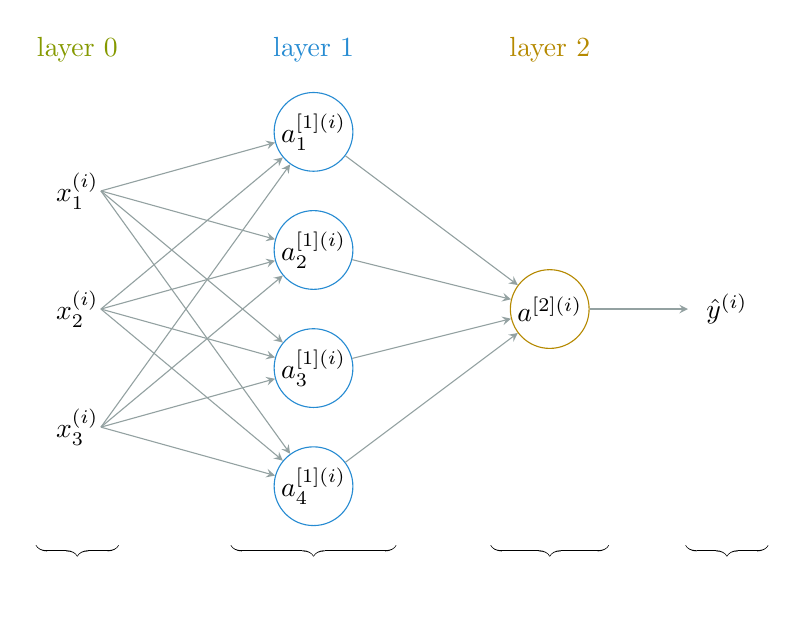
\begin{tikzpicture}[x=1.5cm, y=1.5cm, >=stealth]
		\def\nx{3}
		\def\nu{4}
		% 输入层
		\foreach \i in {1,...,\nx}
			\node[circle, draw=none] (x\i) at (0,2-\i) {$x_\i^{(i)}$};
		\foreach \i in {1,...,\nx}
			\node[coordinate] (lx\i) at (0.2,2-\i) {};
		
		% 隐藏层
		\foreach \h in {1,...,\nu}
			\node[circle, draw=blue, fill=white, inner sep=0pt, minimum size=10mm] (h\h) at (2,2.5-\h) {$a_\h^{[1](i)}$};
		
		% 输出层
		\node[circle, draw=yellow, fill=white, inner sep=0pt, minimum size=10mm] (o) at (4,0) {$a^{[2](i)}$};
	
		% 预测值
		\node[circle, draw=none] (yhat) at (5.5,0) {$\hat{y}^{(i)}$};
		
	
		% 连接
		\foreach \i in {1,...,\nx}
			\foreach \h in {1,...,\nu}
				\draw[->, color=base1] (lx\i) -- (h\h);
		
		\foreach \h in {1,...,\nu}
			\draw[->, color=base1] (h\h) -- (o);
		
		\draw[->, color=base1] (o) -- (yhat);
		
		% 标签
		\def\labely{-2}
		\node [green] at (0,2.2) {layer 0};
		\node [blue] at (2,2.2) {layer 1};
		\node [yellow] at (4,2.2) {layer 2};
		\draw [decorate,decoration={calligraphic brace,amplitude=4pt,mirror}] (-0.35,\labely) -- (0.35,\labely) node [green,midway,yshift=-0.5cm] {输入层};
		\draw [decorate,decoration={calligraphic brace,amplitude=4pt,mirror}] (1.3,\labely) -- (2.7,\labely) node [blue,midway,yshift=-0.5cm] {隐藏层};
		\draw [decorate,decoration={calligraphic brace,amplitude=4pt,mirror}] (3.5,\labely) -- (4.5,\labely) node [yellow,midway,yshift=-0.5cm] {输出层};
		\draw [decorate,decoration={calligraphic brace,amplitude=4pt,mirror}] (5.15,\labely) -- (5.85,\labely) node [red,midway,yshift=-0.5cm] {预测值};
	
	\end{tikzpicture}
	\caption{Shallow Neural Network 浅层神经网络}
	\label{fig:shallow_nn}
\end{figure}

\begin{figure}[h!bt]
	\centering
	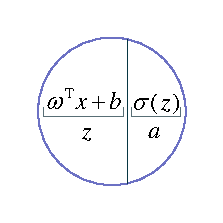
\includegraphics[width=5cm]{node.pdf}
	\caption{单个节点的结构}
	\label{fig:node}
\end{figure}

%%%
\subsection{Activation Functions}
\index{Activation Functions}

常见的激活函数有sigmoid函数、tanh函数、ReLU函数、leaky ReLU函数等,如图 \ref{fig:activation} 所示。对于导数不存在的点,可以使用左导数或右导数代替。

\begin{figure*}[h!bt]
	\centering
	\subfigure[$\mathrm{sigmoid}(z) = \frac{1}{1+\mathrm{e}^{-z}}$]{
		\begin{minipage}[t]{0.5\linewidth}
			\centering
			\includesvg[width=7cm]{activation_sigmoid}
		\end{minipage}
	}%
	\subfigure[$\mathrm{tanh}(z) = \frac{\mathrm{e}^{z} - \mathrm{e}^{-z}}{\mathrm{e}^{z} + \mathrm{e}^{-z}}$]{
		\begin{minipage}[t]{0.5\linewidth}
			\centering
			\includesvg[width=7cm]{activation_tanh}
		\end{minipage}
	}%
	%此处的空行很重要,想让图片在什么地方换行就在代码对应位置空行

	\subfigure[$\mathrm{ReLU}(z) = \max(0, z)$]{
		\begin{minipage}[t]{0.5\linewidth}
			\centering
			\includesvg[width=7cm]{activation_ReLU}
		\end{minipage}
	}%
	\subfigure[$\mathrm{LeakyReLU}(z) = \max(0.01z, z)$]{
		\begin{minipage}[t]{0.5\linewidth}
			\centering
			\includesvg[width=7cm]{activation_LeakyReLU}
		\end{minipage}
	}%
	\centering
	\caption{Activation Functions 激活函数}
	\label{fig:activation}
\end{figure*}

这些激活函数的导数分别为:
\begin{equation}
	\begin{aligned}
		\frac{\mathrm{d}}{\mathrm{d}z}\mathrm{sigmoid}(z) &= \mathrm{sigmoid}(z)\left(1-\mathrm{sigmoid}(z)\right) \\
		\frac{\mathrm{d}}{\mathrm{d}z}\mathrm{tanh}(z) &= 1 - \mathrm{tanh}^2(z) \\
		\frac{\mathrm{d}}{\mathrm{d}z}\mathrm{ReLU}(z) &= 
			\begin{cases}
				0, &z < 0 \\
				1, &z \geqslant 0
			\end{cases}\\
		\frac{\mathrm{d}}{\mathrm{d}z}\mathrm{LeakyReLU}(z) &= 
			\begin{cases}
				0.01, &z < 0 \\
				1, &z \geqslant 0
			\end{cases}
	\end{aligned}
\end{equation}

需要强调的是,激活函数是必要的,如果没有激活函数,那么神经网络的每一层都是线性的,无论有多少层,整个神经网络都相当于一层线性函数,这样就无法解决复杂的问题。

%%%
\subsection{Gradient Descent for Neural Networks}
在训练整个神经网络时,需要对每一层的权重和偏置进行梯度下降,因此需要对每一层的梯度进行计算。

\vspace{0.5\baselineskip}
我们的目标是最小化代价函数$J(W^{[1]}, b^{[1]}, W^{[2]}, b^{[2]}, \cdots, W^{[L]}, b^{[L]})$,其中$L$为神经网络的层数。对于第$l$层,先求出权重和偏置的偏导数,然后再进行梯度下降,即
\begin{equation}
	\begin{aligned}
		W^{[l]} &:= W^{[l]} - \alpha \frac{\mathrm{d}J}{\mathrm{d}W^{[l]}} \\
		b^{[l]} &:= b^{[l]} - \alpha \frac{\mathrm{d}J}{\mathrm{d}b^{[l]}}
	\end{aligned}
\end{equation}

%%%
\subsection{Backpropagation}
\index{Backpropagation}
在神经网络中,梯度下降用到了\textbf{反向传播算法(Backpropagation)},该算法的基本思想是,先计算代价函数对输出层的梯度,然后再反向传播到每一层,计算每一层$W$和$b$的梯度。
需要注意,在每一轮梯度下降中,\textbf{所有的$X$, $Y$, $Z$, $A$都是已知的常量,而$W$, $b$是需要更新的}。

在推导过程中,需要补充一些矩阵导数运算的知识,参见附录 \ref{sec:matrix_derivative}。以下过程中使用的符号如表 \ref{tab:notations} 所示。

\vspace{0.5\baselineskip}
对于第$l$层,\colorbox{LemonChiffon}{已知$\dfrac{\mathrm{d}J}{\mathrm{d}A^{[l]}}$}和关系
\begin{equation}
	\vcenter{\hbox{\tikzmarknode{Zl}{$Z^{[l]}$}}} \vcenter{\hbox{$\vphantom{1}=\vphantom{1}$\tikzmarknode{Wl}{$W^{[l]}$}\tikzmarknode{Al-1}{$A^{[l-1]}$}$\vphantom{1}+\vphantom{1}$}} \begin{bmatrix} b^{[l]} & b^{[l]} & \cdots & b^{[l]} \end{bmatrix}_{\substack{\scriptstyle n^{[l]}\times m}}
	\annotate[yshift=1em]{above}{Zl}{$n^{[l]}\times m$}
	\annotate[yshift=-1em]{below,left}{Wl}{$n^{[l]}\times n^{[l-1]}$}
	\annotate[yshift=-1em]{below}{Al-1}{$n^{[l-1]}\times m$}
	\label{eq:backpropagation_known_1}
\end{equation}
\begin{equation}
	\tikzmarknode{Al}{A^{[l]}} = g^{[l]}(\tikzmarknode{Zl2}{Z^{[l]}})
	\vspace{1em}
	\label{eq:backpropagation_known_2}
	\annotatetwo[yshift=-1em]{below,label below}{Al}{Zl2}{$n^{[l]}\times m$}
\end{equation}
\colorbox{LemonChiffon}{要计算$\dfrac{\mathrm{d}J}{\mathrm{d}A^{[l-1]}}$, $\dfrac{\mathrm{d}J}{\mathrm{d}W^{[l]}}$和$\dfrac{\mathrm{d}J}{\mathrm{d}b^{[l]}}$}。
根据结论\eqref{eq:matrix_derivative_conclusion1},式\eqref{eq:backpropagation_known_1}可推出下面的关系
\begin{align}
	\frac{\mathrm{d}J}{\mathrm{d}W^{[l]}} &= \frac{\mathrm{d}J}{\mathrm{d}Z^{[l]}} A^{[l-1] \mathrm{T}} 
	\label{eq:backpropagation_conc_1} \\
	\frac{\mathrm{d}J}{\mathrm{d}A^{[l-1]}} &= W^{[l] \mathrm{T}} \frac{\mathrm{d}J}{\mathrm{d}Z^{[l]}}
	\label{eq:backpropagation_conc_2}
\end{align}
根据结论\eqref{eq:matrix_derivative_conclusion2},式\eqref{eq:backpropagation_known_2}表明
\begin{equation}
	\frac{\mathrm{d}J}{\mathrm{d}Z^{[l]}} = g^{[l]'}(Z^{[l]}) \odot \frac{\mathrm{d}J}{\mathrm{d}A^{[l]}}
	\label{eq:backpropagation_conc_3}
\end{equation}
由于$b^{[l]}$在计算时进行了维度扩充,$\dfrac{\mathrm{d}J}{\mathrm{d}b^{[l]}}$的求取较为特殊。首先考虑第$i$个样本,上面的关系可以写成
\begin{equation}
	z^{[l](i)} = W^{[l]} a^{[l-1](i)} + b^{[l]}
	\label{eq:backpropagation_known_1_sample}
\end{equation}
根据结论\eqref{eq:matrix_derivative_conclusion1},式\eqref{eq:backpropagation_known_1_sample}可推出下面的关系
\begin{equation}
	\frac{\mathrm{d}L^{(i)}}{\mathrm{d}b^{[l]}} = \frac{\mathrm{d}L^{(i)}}{\mathrm{d}z^{[l](i)}}
	\label{eq:backpropagation_known_1_sample_derivative}
\end{equation}
一般认为各个样本间相互独立,从而有
\begin{equation}
	\frac{\mathrm{d}L^{(\textcolor{blue}{i})}}{\mathrm{d}z^{[l](\textcolor{red}{j})}}=0
	, \quad \textcolor{blue}{i} \neq \textcolor{red}{j}, \quad 0 \leqslant l \leqslant L
	\label{eq:backpropagation_known_1_sample_derivative_independent}
\end{equation}
回顾代价函数的定义
\begin{equation}
	J = \frac{1}{m} \sum_{i=1}^{m} L^{(i)}
\end{equation}
结合式\eqref{eq:backpropagation_known_1_sample_derivative_independent},可得
\begin{equation}
	\begin{aligned}
		\frac{\mathrm{d}J}{\mathrm{d}z^{[l](i)}} 
		&= \frac{1}{m}  \sum_{\textcolor{red}{j}=1}^{m} \frac{\mathrm{d}L^{(\textcolor{red}{j})}}{\mathrm{d}z^{[l](i)}} \\
		&= \frac{1}{m}  \left( \sum_{\substack{1 \leqslant \textcolor{red}{j} \leqslant m \\ \textcolor{red}{j} \neq i}} \tikzmarknode{zero}{\frac{\mathrm{d}L^{(\textcolor{red}{j})}}{\mathrm{d}z^{[l](i)}}} + \frac{\mathrm{d}L^{(i)}}{\mathrm{d}z^{[l](i)}} \right) \\
		&= \frac{1}{m} \frac{\mathrm{d}L^{(i)}}{\mathrm{d}z^{[l](i)}} \\
	\end{aligned}
	\annotate[yshift=1em]{above}{zero}{equals 0}
\end{equation}
两边乘$m$即得
\begin{equation}
	\frac{\mathrm{d}L^{(i)}}{\mathrm{d}z^{[l](i)}} = m \frac{\mathrm{d}J}{\mathrm{d}z^{[l](i)}}
\end{equation}
结合式\eqref{eq:backpropagation_known_1_sample_derivative}和代价函数定义,可推知
\begin{equation}
	\begin{aligned}
		\frac{\mathrm{d}J}{\mathrm{d}b^{[l]}} 
		&= \frac{1}{m} \sum_{i=1}^{m} \frac{\mathrm{d}L^{(i)}}{\mathrm{d}b^{[l]}} \\
		&= \frac{1}{m} \sum_{i=1}^{m} \frac{\mathrm{d}L^{(i)}}{\mathrm{d}z^{[l](i)}} \\
		&= \frac{1}{m} \sum_{i=1}^{m} m \frac{\mathrm{d}J}{\mathrm{d}z^{[l](i)}} \\
		&= \tikzmarknode{db}{\sum_{i=1}^{m} \frac{\mathrm{d}J}{\mathrm{d}z^{[l](i)}}}
	\label{eq:backpropagation_conc_4}
	\end{aligned}
	\vspace{2em}
	\annotate[yshift=0em]{below}{db}{相当于$\dfrac{\mathrm{d}J}{\mathrm{d}Z^{[l]}}$沿水平方向求和}
\end{equation}
综合式\eqref{eq:backpropagation_conc_3}, \eqref{eq:backpropagation_conc_2}, \eqref{eq:backpropagation_conc_1}, 和\eqref{eq:backpropagation_conc_4},可得
\footnote{此推导结果与课程不同,主要区别是系数$\dfrac{1}{m}$的位置不同。课程中将$\dfrac{1}{m}$放在了所有的$\dfrac{\mathrm{d}J}{\mathrm{d}W}$和$\dfrac{\mathrm{d}J}{\mathrm{d}b}$处,但实际上应该位于$\dfrac{\mathrm{d}J}{\mathrm{d}A^{[L]}}$处并反向传播至各层。但是这不会影响最终的结果。}
\begin{align}
	\frac{\mathrm{d}J}{\mathrm{d}Z^{[l]}} &= g^{[l]'}(Z^{[l]}) \odot \frac{\mathrm{d}J}{\mathrm{d}A^{[l]}} \\
	\frac{\mathrm{d}J}{\mathrm{d}A^{[l-1]}} &= W^{[l] \mathrm{T}} \frac{\mathrm{d}J}{\mathrm{d}Z^{[l]}} \\
	\frac{\mathrm{d}J}{\mathrm{d}W^{[l]}} &= \frac{\mathrm{d}J}{\mathrm{d}Z^{[l]}} A^{[l-1] \mathrm{T}} \label{eq:dw_real} \\
	\frac{\mathrm{d}J}{\mathrm{d}b^{[l]}} &= \sum_{i=1}^{m} \frac{\mathrm{d}J}{\mathrm{d}z^{[l](i)}} \label{eq:db_real}
\end{align}
将以上结论写成伪代码形式,
\begin{align}
	\mathtt{dZ^{\textcolor{Magenta}{[}l\textcolor{Magenta}{]}}} &= \mathtt{g^{\textcolor{Magenta}{[}l\textcolor{Magenta}{]}'}\textcolor{yellow}{(}Z^{\textcolor{Magenta}{[}l\textcolor{Magenta}{]}}\textcolor{yellow}{)} \,\tikzmarknode{star}{*}\, dA^{\textcolor{Magenta}{[}l\textcolor{Magenta}{]}}} \\
	\mathtt{dA^{\textcolor{Magenta}{[}l-\textcolor{green}{1}\textcolor{Magenta}{]}}} &= \mathtt{W^{\textcolor{Magenta}{[}l\textcolor{Magenta}{]} T} dZ^{\textcolor{Magenta}{[}l\textcolor{Magenta}{]}}} \\
	\mathtt{dW^{\textcolor{Magenta}{[}l\textcolor{Magenta}{]}}} &= \mathtt{dZ^{\textcolor{Magenta}{[}l\textcolor{Magenta}{]}} A^{\textcolor{Magenta}{[}l-\textcolor{green}{1}\textcolor{Magenta}{]}T}} \label{eq:dw} \\
	\mathtt{db^{\textcolor{Magenta}{[}l\textcolor{Magenta}{]}}} &= \mathtt{np.sum\textcolor{yellow}{(}dZ^{\textcolor{Magenta}{[}l\textcolor{Magenta}{]}}, axis=\textcolor{green}{1}, keepdims=\textcolor{blue}{True}\textcolor{yellow}{)}} \label{eq:db}
	\annotate[yshift=1.5em]{above}{star}{element-wise multiplication}
\end{align}

下面来\colorbox{LemonChiffon}{计算$\dfrac{\mathrm{d}J}{\mathrm{d}A^{[L]}}$}。回顾损失函数(交叉熵损失函数)的定义
\begin{equation}
	L^{(i)} = -\left[y^{(i)} \log \hat{y}^{(i)} + (1 - y^{(i)}) \log (1 - \hat{y}^{(i)})\right]
\end{equation}
对其求导,可得
\begin{equation}
	\frac{\mathrm{d}L^{(i)}}{\mathrm{d}\hat{y}^{(i)}} = -\frac{y^{(i)}}{\hat{y}^{(i)}} + \frac{1 - y^{(i)}}{1 - \hat{y}^{(i)}}
\end{equation}
从而
\begin{equation}
	\frac{\mathrm{d}J}{\mathrm{d}\hat{y}^{(i)}} 
	= \frac{1}{m} \sum_{\textcolor{red}{j}=1}^{m} \frac{\mathrm{d}L^{(\textcolor{red}{j})}}{\mathrm{d}\hat{y}^{(i)}} 
	= \frac{1}{m} \frac{\mathrm{d}L^{(i)}}{\mathrm{d}\hat{y}^{(i)}} 
	= \frac{1}{m} \left(-\frac{y^{(i)}}{\hat{y}^{(i)}} + \frac{1 - y^{(i)}}{1 - \hat{y}^{(i)}}\right)
\end{equation}
将各个样本的值写在一起,可得
\begin{equation}
	\frac{\mathrm{d}J}{\mathrm{d}\hat{Y}} 
	= \begin{bmatrix} \dfrac{\mathrm{d}J}{\mathrm{d}\hat{y}^{(1)}} & \dfrac{\mathrm{d}J}{\mathrm{d}\hat{y}^{(2)}} & \cdots & \dfrac{\mathrm{d}J}{\mathrm{d}\hat{y}^{(m)}} \end{bmatrix}
	= \frac{1}{m} \left(-\frac{Y}{\hat{Y}} + \frac{1 - Y}{1 - \hat{Y}}\right)
\end{equation}
即
\begin{equation}
	\frac{\mathrm{d}J}{\mathrm{d}A^{[L]}} 
	= \frac{1}{m} \left(-\frac{Y}{A^{[L]}} + \frac{1 - Y}{1 - A^{[L]}}\right)
\end{equation}
写成伪代码形式为
\begin{equation}
	\mathtt{dA^{\textcolor{Magenta}{[}L\textcolor{Magenta}{]}}} = \mathtt{\frac{1}{m} \textcolor{blue}{(}np.divide\textcolor{yellow}{(}Y, A^{\textcolor{Magenta}{[}L\textcolor{Magenta}{]}}\textcolor{yellow}{)} - np.divide\textcolor{yellow}{(}1 - Y, 1 - A^{\textcolor{Magenta}{[}L\textcolor{Magenta}{]}}\textcolor{yellow}{)}}\textcolor{blue}{)} \label{eq:da}
\end{equation}
\textbf{从输出层开始,先得到$\dfrac{\mathrm{d}J}{\mathrm{d}A^{[L]}}$(也就是$\dfrac{\mathrm{d}J}{\mathrm{d}\hat{Y}}$),然后逐层向前计算,直到第$1$层,即可得到所有的梯度。}

\vspace{\baselineskip}
对于本节要构建的浅层神经网络,使用的激活函数为sigmoid函数,
\begin{equation}
	A = g(Z) \quad \Rightarrow \quad g'(Z) = A(1-A)
\end{equation}
利用
\begin{equation}
	\frac{\mathrm{d}J}{\mathrm{d}A^{[2]}} 
	= \frac{1}{m} \left(-\frac{Y}{A^{[2]}} + \frac{1 - Y}{1 - A^{[2]}}\right)
\end{equation}
可得
\begin{align}
	\frac{\mathrm{d}J}{\mathrm{d}Z^{[2]}} &= A^{[2]}(1-A^{[2]}) \odot \frac{\mathrm{d}J}{\mathrm{d}A^{[2]}} = \frac{1}{m}(A^{[2]}-Y) \\
	\frac{\mathrm{d}J}{\mathrm{d}A^{[1]}} &= W^{[2] \mathrm{T}} \frac{\mathrm{d}J}{\mathrm{d}Z^{[2]}} \\
	\frac{\mathrm{d}J}{\mathrm{d}W^{[2]}} &= \frac{\mathrm{d}J}{\mathrm{d}Z^{[2]}} A^{[1] \mathrm{T}} \\
	\frac{\mathrm{d}J}{\mathrm{d}b^{[2]}} &= \sum_{i=1}^{m} \frac{\mathrm{d}J}{\mathrm{d}z^{[2](i)}}
\end{align}
进而
\begin{align}
	\frac{\mathrm{d}J}{\mathrm{d}Z^{[1]}} &= A^{[1]}(1-A^{[1]}) \odot \frac{\mathrm{d}J}{\mathrm{d}A^{[1]}} = W^{[2] \mathrm{T}} \frac{\mathrm{d}J}{\mathrm{d}Z^{[2]}} \odot A^{[1]}(1-A^{[1]}) \\
	\frac{\mathrm{d}J}{\mathrm{d}W^{[1]}} &= \frac{\mathrm{d}J}{\mathrm{d}Z^{[1]}} A^{[0] \mathrm{T}} = \frac{\mathrm{d}J}{\mathrm{d}Z^{[1]}} X^{\mathrm{T}} \\
	\frac{\mathrm{d}J}{\mathrm{d}b^{[1]}} &= \sum_{i=1}^{m} \frac{\mathrm{d}J}{\mathrm{d}z^{[1](i)}}
\end{align}
总结为伪代码形式
\begin{align}
	\mathtt{dZ^{\textcolor{Magenta}{[}2\textcolor{Magenta}{]}}} &= \mathtt{\frac{1}{m} \textcolor{yellow}{(}A^{\textcolor{Magenta}{[}2\textcolor{Magenta}{]}}-Y\textcolor{yellow}{)}} \\
	\mathtt{dW^{\textcolor{Magenta}{[}2\textcolor{Magenta}{]}}} &= \mathtt{dZ^{\textcolor{Magenta}{[}2\textcolor{Magenta}{]}} A^{\textcolor{Magenta}{[}1\textcolor{Magenta}{]}T}} \\
	\mathtt{db^{\textcolor{Magenta}{[}2\textcolor{Magenta}{]}}} &= \mathtt{np.sum\textcolor{yellow}{(}dZ^{\textcolor{Magenta}{[}2\textcolor{Magenta}{]}}, axis=\textcolor{green}{1}, keepdims=\textcolor{blue}{True}\textcolor{yellow}{)}} \\
	\mathtt{dZ^{\textcolor{Magenta}{[}1\textcolor{Magenta}{]}}} &= \mathtt{W^{\textcolor{Magenta}{[}2\textcolor{Magenta}{]}T} dZ^{\textcolor{Magenta}{[}2\textcolor{Magenta}{]}} * A^{\textcolor{Magenta}{[}1\textcolor{Magenta}{]}}\textcolor{yellow}{(}1 - A^{\textcolor{Magenta}{[}1\textcolor{Magenta}{]}}\textcolor{yellow}{)}} \\
	\mathtt{dW^{\textcolor{Magenta}{[}1\textcolor{Magenta}{]}}} &= \mathtt{dZ^{\textcolor{Magenta}{[}1\textcolor{Magenta}{]}} X^T} \\
	\mathtt{db^{\textcolor{Magenta}{[}1\textcolor{Magenta}{]}}} &= \mathtt{np.sum\textcolor{yellow}{(}dZ^{\textcolor{Magenta}{[}1\textcolor{Magenta}{]}}, axis=\textcolor{green}{1}, keepdims=\textcolor{blue}{True}\textcolor{yellow}{)}}
\end{align}

%%%
\subsection{Random Initialization}
在神经网络中,权重的初始值不能全部为$0$,否则会导致神经网络各层的神经元进行相同的计算,无法正常工作。

\vspace{0.5\baselineskip}
在神经网络中,权重的初始值通常使用随机数生成,如
\begin{equation}
	W^{[l]} = \mathtt{np.random.randn}(n^{[l]}, n^{[l-1]}) \times 0.01
\end{equation}
其中,$\mathtt{np.random.randn}(n^{[l]}, n^{[l-1]})$表示生成一个$n^{[l]} \times n^{[l-1]}$的随机矩阵,每个元素都是从均值为$0$,方差为$1$的高斯分布中随机取值,然后再乘以$0.01$。乘上$0.01$是为了保证$W^{[l]}$的值不会太大,在初始时在激活函数梯度较大处(靠近$0$)进行训练,否则会导致激活函数的输入值过大,从而导致梯度消失或梯度爆炸。\\
对于偏置,可以直接使用$0$初始化,
\begin{equation}
	b^{[l]} = \mathtt{np.zeros}((n^{[l]}, 1))
\end{equation}

	% % % % % % % % % %
	\part{Projects}
	
	\chapter[短章名]{这是一个充分长的章名, 强势占用三行没商量.}
	如果章名过长, 可以在目录和天眉以另外设置的短章名显示, 方式和 \LaTeX 的标准文档类 \textsf{book} 相同.

	\section{长度正常的节名}
	复数 $\tau$ 的虚部记为 $\Im(\tau)$. 自然对数记为 $\log$.
	
	\begin{convention}
		本节记 Poincaré 上半平面为
		\[ \mathcal{H} := \left\{ \tau \in \mathbb{C}: \Im(\tau) > 0 \right\}. \]
		按例记 $q := e^{2\pi i \tau}$.	\emph{Dedekind $\eta$ 函数}定义为无穷乘积
		\[ \eta(\tau) := e^{2\pi i \tau/24} \prod_{n=1}^\infty (1 - q^n), \quad \tau \in \mathcal{H}. \]
	\end{convention}
	由分析学常识易见此无穷乘积绝对收敛. 进一步, $\eta$ 在 $\mathcal{H}$ 上全纯无零点; 此外 $\eta$ 的对数导数为
	\[ \frac{\mathrm{d}}{\mathrm{d}\tau} \log \eta (\tau) := \frac{\eta'(\tau)}{\eta(\tau)} = \frac{\pi i}{12} - 2\pi i \sum_{n=1}^\infty \frac{n q^n}{1 - q^n}. \]
	
	\begin{example}
		在右半复平面上定义 $\sqrt{z} := \exp(\log|z| + i\arg(z))$, 其中幅角取 $\arg(z) \in \left[-\frac{\pi}{2}, \frac{\pi}{2}\right]$. 则
		\[ \eta\left( \frac{-1}{\tau} \right) = \sqrt{-i\tau} \cdot \eta(\tau), \quad \tau \in \mathcal{H}. \]
	\end{example}
	\begin{proof}
		应用 Eisenstein 级数 $E_2$ 的性质, 将对数导数 $\frac{\mathrm{d}}{\mathrm{d} \tau} \log\eta(\tau)$ 整理为
		\begin{multline*}
			\frac{\pi i}{12} - 2\pi i \sum_{d \geq 1} \frac{dq^d}{1- q^d} = \frac{\pi i}{12} - 2\pi i \sum_{d \geq 1} \sum_{k \geq 1} d q^{dk} \\
			\stackrel{n := dk}{=} \frac{\pi i}{12} - 2\pi i \sum_{n \geq 1} \sigma_1(n) q^n = \dfrac{\pi i}{12} \cdot E_2(\tau),
		\end{multline*}
		若改为对 $\tau \mapsto \eta(\frac{-1}{\tau})$ 求对数导数, 再应用 $E_2$ 的函数方程, 产物则是
		\[ \tau^{-2} \cdot \frac{\pi i}{12} \cdot E_2\left(\frac{-1}{\tau}\right) = \frac{\pi i}{12} \left(E_2(\tau) + \frac{12}{2\pi i \tau} \right). \]
		对 $\sqrt{-i\tau}$ 求对数导数给出 $\frac{1}{2} \frac{\mathrm{d}}{\mathrm{d}\tau} \log(-i\tau) = \dfrac{1}{2\tau} = \dfrac{\pi i}{12} \cdot \dfrac{12}{2 \pi i \tau}$. 与上式对比即见
		\begin{align*}
			\frac{\mathrm{d}}{\mathrm{d} \tau} \log \eta\left( \frac{-1}{\tau} \right) & = \frac{\mathrm{d}}{\mathrm{d} \tau} \log \sqrt{-i\tau} + \frac{\mathrm{d}}{\mathrm{d} \tau} \log \eta(\tau)  \\
			& = \frac{\mathrm{d}}{\mathrm{d} \tau} \log \left( \sqrt{-i\tau} \cdot \eta(\tau) \right).
		\end{align*}
		故存在 $c \in \mathbb{C}^\times$ 使得 $\eta\left(\frac{-1}{\tau}\right) = c \sqrt{-i\tau} \cdot \eta(\tau)$; 因为 $\eta(i) \neq 0$, 代入 $\tau = i$ 可知 $c = 1$.
	\end{proof}

	著名的 Euler 五边形数定理写作
	\begin{equation}\label{eqn:pentagonal-number}
		\sum_{n \in \mathbb{Z}} (-1)^n q^{(3n^2 + n)/2} = \prod_{n \geq 1} (1 - q^n);
	\end{equation}
	留意到 $3n^2 + n \equiv 0 \pmod 2$ 恒成立. 将 $\frac{3n^2 + n}{2} = \frac{(6n+1)^2 - 1}{24}$ 代入 \eqref{eqn:pentagonal-number}, 即可导出 $\eta$ 的 Fourier 展开
	\begin{equation*}
		\eta(\tau) = \sum_{n \in \mathbb{Z}} (-1)^n q^{ \frac{1}{24} \cdot (6n + 1)^2}, \quad q^{1/24} := e^{2\pi i \tau /24}.
	\end{equation*}

	\section[短节名]{
		四十男儿学干谒,朝游江淮暮吴越。漫将衣食累朱门,讵有文章动金阙。
		倦游屡岁赋归欤,故人相值还唏嘘。劝我莫作千里客,留我共读三冬书。
		忆别吴阊一年久,为我糟床压春酒。入座争迎作赋才,当筵更觅弹筝手。
		酒酣慷慨唤奈何,风光一往如流波。女坟湖北莺犹少,短簿祠南雨正多。
		君家奇书一千轴,锦袱牙签光历碌。愿随潘左伴青缃,羞与金张斗华毂。
		嗟余短鬓日苍浪,太息忧来未可忘。鼓挝马槊差亦得,若问读书非我长。}
	原诗作者: [清] 陈维崧.

	不鼓励使用过长的节名. 同样地, 可以在目录和天眉以另外设置的短节名显示, 方式和 \LaTeX 的标准文档类 \textsf{book} 相同.

	\begin{Exercises}
		\item 造访兰州. \begin{hint} 低碳出行, 请乘坐火车. \end{hint}
		\item 造访祁连山.
	\end{Exercises}

	% % % % % % % % % %
	\part{Supplements}

	\appendix
\chapter{Mathmatical}

%%%%
\section{Matrix derivative}
\label{sec:matrix_derivative}
\index{Matrix derivative}

\begin{wenxintishi}
	在本节中,为便于区分,用粗体大写字母表示矩阵,用粗体小写字母表示向量,用普通小写字母表示标量。这些表示与正文不同。
\end{wenxintishi}

矩阵微积分的表示通常有两种符号约定,分别是\textbf{分子布局(Numerator Layout)}和\textbf{分母布局(Denominator Layout)}\cite{matrix_cookbook}。下面将分别介绍这两种符号约定。

%%%
\subsection{标量关于向量的偏导数}
如果一个标量函数$f(\bm{x})$的自变量是一个$n$维向量$\bm{x}$,那么这个标量函数就可以对这个向量$\bm{x}$求偏导数。

在分子布局下,这个偏导数是一个行向量,其第$i$个元素是$f(\bm{x})$对$\bm{x}$的第$i$个元素的偏导数,即
\begin{equation}
	\frac{\partial f(\bm{x})}{\partial \bm{x}}
	=\left[\frac{\partial f(\bm{x})}{\partial x_1},\frac{\partial f(\bm{x})}{\partial x_2},\cdots,\frac{\partial f(\bm{x})}{\partial x_n}\right]_{\substack{\scriptstyle 1\times n}}
\end{equation}
而在分母布局下,这个偏导数是一个列向量,其第$i$个元素是$f(\bm{x})$对$\bm{x}$的第$i$个元素的偏导数,即
\begin{equation}
	\frac{\partial f(\bm{x})}{\partial \bm{x}}
	=\begin{bmatrix}
		\dfrac{\partial f(\bm{x})}{\partial x_1}\\[2ex]
		\dfrac{\partial f(\bm{x})}{\partial x_2}\\[2ex]
		\vdots\\[2ex]
		\dfrac{\partial f(\bm{x})}{\partial x_n}
	\end{bmatrix}_{\substack{\scriptstyle n\times 1}}
\end{equation}

%%%
\subsection{向量关于标量的偏导数}
如果一个$m$维向量函数$\bm{f}(x)$的自变量是一个标量$x$,那么这个向量函数就可以对这个标量$x$求偏导数。


在分子布局下,这个偏导数是一个列向量,其第$i$个元素是$\bm{f}(x)$对$x$的偏导数,即
\begin{equation}
	\frac{\partial \bm{f}(x)}{\partial x}
	=\begin{bmatrix}
		\dfrac{\partial f_1(x)}{\partial x}\\[2ex]
		\dfrac{\partial f_2(x)}{\partial x}\\[2ex]
		\vdots\\[2ex]
		\dfrac{\partial f_m(x)}{\partial x}
	\end{bmatrix}_{\substack{\scriptstyle m\times 1}}
\end{equation}
而在分母布局下,这个偏导数是一个行向量,其第$i$个元素是$\bm{f}(x)$对$x$的偏导数,即
\begin{equation}
	\frac{\partial \bm{f}(x)}{\partial x}
	=\left[\frac{\partial f_1(x)}{\partial x},\frac{\partial f_2(x)}{\partial x},\cdots,\frac{\partial f_m(x)}{\partial x}\right]_{\substack{\scriptstyle 1\times m}}
\end{equation}

%%%
\subsection{向量关于向量的偏导数}
如果一个$m$维向量函数$\bm{f}(\bm{x})$的自变量是一个$n$维向量$\bm{x}$,那么这个向量函数就可以对这个向量$\bm{x}$求偏导数。

在分子布局下,这个偏导数是一个$m\times n$维矩阵,其第$i$行第$j$列的元素是$f_i(\bm{x})$对$\bm{x}$的第$j$个元素的偏导数,即
\begin{equation}
	\frac{\partial \bm{f}(\bm{x})}{\partial \bm{x}}
	=\left[\frac{\partial \bm{f}(\bm{x})}{\partial x_1},\frac{\partial \bm{f}(\bm{x})}{\partial x_2},\cdots,\frac{\partial \bm{f}(\bm{x})}{\partial x_n}\right]
	=\begin{bmatrix}
		\dfrac{\partial f_1(\bm{x})}{\partial x_1}&\dfrac{\partial f_1(\bm{x})}{\partial x_2}&\cdots&\dfrac{\partial f_1(\bm{x})}{\partial x_n}\\[2ex]
		\dfrac{\partial f_2(\bm{x})}{\partial x_1}&\dfrac{\partial f_2(\bm{x})}{\partial x_2}&\cdots&\dfrac{\partial f_2(\bm{x})}{\partial x_n}\\[2ex]
		\vdots&\vdots&\ddots&\vdots\\[2ex]
		\dfrac{\partial f_m(\bm{x})}{\partial x_1}&\dfrac{\partial f_m(\bm{x})}{\partial x_2}&\cdots&\dfrac{\partial f_m(\bm{x})}{\partial x_n}
	\end{bmatrix}_{\substack{\scriptstyle m\times n}}
\end{equation}
而在分母布局下,这个偏导数是一个$n\times m$维矩阵,其第$i$行第$j$列的元素是$f_j(\bm{x})$对$\bm{x}$的第$i$个元素的偏导数,即
\begin{equation}
	\frac{\partial \bm{f}(\bm{x})}{\partial \bm{x}}
	=\left[\frac{\partial f_1(\bm{x})}{\partial \bm{x}},\frac{\partial f_2(\bm{x})}{\partial \bm{x}},\cdots,\frac{\partial f_m(\bm{x})}{\partial \bm{x}}\right]
	=\begin{bmatrix}
		\dfrac{\partial f_1(\bm{x})}{\partial x_1}&\dfrac{\partial f_2(\bm{x})}{\partial x_1}&\cdots&\dfrac{\partial f_m(\bm{x})}{\partial x_1}\\[2ex]
		\dfrac{\partial f_1(\bm{x})}{\partial x_2}&\dfrac{\partial f_2(\bm{x})}{\partial x_2}&\cdots&\dfrac{\partial f_m(\bm{x})}{\partial x_2}\\[2ex]
		\vdots&\vdots&\ddots&\vdots\\[2ex]
		\dfrac{\partial f_1(\bm{x})}{\partial x_n}&\dfrac{\partial f_2(\bm{x})}{\partial x_n}&\cdots&\dfrac{\partial f_m(\bm{x})}{\partial x_n}
	\end{bmatrix}_{\substack{\scriptstyle n\times m}}
\end{equation}

一个小结论是,当使用分子布局时,将分子看作列向量,结果的行数与分子相同;而当使用分母布局时,将分母看作列向量,结果的行数与分母相同。

%%%
\subsection{标量关于矩阵的偏导数}
\footnote{本节内容参考了\cite{matrix_derivative}}

在深度学习中,代价函数是一个标量函数,而神经网络的参数通常是一个矩阵。因此,需要求标量函数对矩阵的偏导数。

标量对矩阵求导,可以看作是标量对矩阵的每个元素求导,然后将结果组合成一个矩阵。结果的维度应当与被求导矩阵的维度相同,便于进行梯度下降,故应采用分母布局。本节的内容从这里开始均采用\textcolor{red}{分母布局}。

一元微积分中的导数(标量对标量的导数)满足
\begin{equation}
	\mathrm{d}f 
	= \frac{\partial f}{\partial x}\mathrm{d}x
	= \langle \frac{\partial f}{\partial x}, \mathrm{d}x \rangle
\end{equation}
其中$\langle \bm{u}, \bm{v} \rangle$表示$\bm{u}$与$\bm{v}$的内积。
在多元微积分(标量对向量的导数)中,这个关系可以推广为
\begin{equation}
	\mathrm{d}f
	= \sum_{i=1}^{n}{\frac{\partial f}{\partial x_i}\mathrm{d}x_i} 
	= {\frac{\partial f}{\partial \bm{x}}}^{\mathrm{T}}\mathrm{d}\bm{x}
	= \langle \frac{\partial f}{\partial \bm{x}}, \mathrm{d}\bm{x} \rangle
\end{equation}
类似地,标量对矩阵的导数与微分的关系可以推广为
\begin{equation}
	\mathrm{d}f
	= \langle \frac{\partial f}{\partial \bm{X}}, \mathrm{d}\bm{X} \rangle
	\label{eq:scalar_matrix_derivative}
\end{equation}
两个大小相同矩阵的内积可以表示为
\begin{equation}
	\langle \bm{A}, \bm{B} \rangle 
	= \sum_{i=1}^{m}{\sum_{j=1}^{n}{\frac{\partial f}{\partial x_{ij}}\mathrm{d}x_{ij}}} 
	= \mathrm{tr}(\bm{A}^{\mathrm{T}}\bm{B})
\end{equation}
故式\eqref{eq:scalar_matrix_derivative}可以表示为
\begin{equation}
	\eqnmarkbox[WildStrawberry]{scalar_matrix_derivative_trace}{
	\mathrm{d}f 
	= \mathrm{tr}\left({\frac{\partial f}{\partial \bm{X}}}^{\mathrm{T}}\mathrm{d}\bm{X}\right)
	}
	\label{eq:scalar_matrix_derivative_trace}
\end{equation}
这便是标量对矩阵求导与微分的关系。只要满足式\eqref{eq:scalar_matrix_derivative_trace}的关系,就能得到标量对矩阵的导数。

\vspace{0.5\baselineskip}
下面列出几条常见的矩阵微分的运算法则。注意$\odot$表示Hadamard积,即对应元素相乘。
\begin{subequations}
	\begin{align}
		\mathrm{d}(\bm{X}\pm \bm{Y}) &= \mathrm{d}\bm{X} \pm \mathrm{d}\bm{Y} 
		\label{eq:matrix_derivative_add_sub} \\
		\mathrm{d}(\bm{XY}) &= \mathrm{d}\bm{X}\cdot \bm{Y} + \bm{X}\cdot \mathrm{d}\bm{Y}
		\label{eq:matrix_derivative_mul} \\
		\mathrm{d}(\bm{X}^{\mathrm{T}}) &= (\mathrm{d}\bm{X})^{\mathrm{T}}
		\label{eq:matrix_derivative_transpose} \\
		\mathrm{d}(\bm{X}^{-1}) &= -\bm{X}^{-1}\mathrm{d}\bm{X}\bm{X}^{-1}
		\label{eq:matrix_derivative_inverse} \\
		\mathrm{d}(\bm{X}\odot \bm{Y}) &= \mathrm{d}\bm{X}\odot \bm{Y} + \bm{X}\odot \mathrm{d}\bm{Y}
		\label{eq:matrix_derivative_hadamard} \\
		\mathrm{d}\left(g(\bm{X})\right) &= g'(\bm{X}) \odot \mathrm{d}\bm{X}
		\label{eq:matrix_derivative_hadamard2}
	\end{align}
\end{subequations}

对于矩阵的迹(trace)运算,有以下常用的性质,在后面的推导中会用到。
\begin{subequations}
	\begin{align}
		a &= \mathrm{tr}(a)
		\label{eq:matrix_trace_scalar} \\
		\mathrm{tr}(\bm{A}^{\mathrm{T}}) &= \mathrm{tr}(\bm{A})
		\label{eq:matrix_trace_transpose} \\
		\mathrm{tr}(\bm{A}\pm\bm{B}) &= \mathrm{tr}(\bm{A}) \pm \mathrm{tr}(\bm{B})
		\label{eq:matrix_trace_add_sub} \\
		\mathrm{tr}(\bm{AB}) &= \mathrm{tr}(\bm{BA})
		\label{eq:matrix_trace_mul} \\
		\mathrm{tr}\left(\bm{A}^{\mathrm{T}}(\bm{B} \odot \bm{C})\right) &= \mathrm{tr}\left((\bm{A} \odot \bm{B})^{\mathrm{T}}\bm{C}\right)
		\label{eq:matrix_trace_hadamard}
	\end{align}
\end{subequations}

在复合情况下,为了避免矩阵对矩阵求导,尽量不要使用链式法则,而是使用微分的性质\eqref{eq:scalar_matrix_derivative_trace},通过迹运算的变形来求解。

\begin{example}\label{example:matrix_derivative1}
\vspace{0.5\baselineskip}
\colorbox{LemonChiffon}{已知$\dfrac{\partial f}{\partial \bm{Y}}$和$\bm{Y}=\bm{A}\bm{X}\bm{B}$,求$\dfrac{\partial f}{\partial \bm{X}}$}。
根据式\eqref{eq:scalar_matrix_derivative_trace},有
\begin{equation}
	\mathrm{d}f = \mathrm{tr}\left({\frac{\partial f}{\partial \bm{Y}}}^{\mathrm{T}}\mathrm{d}\bm{Y}\right)
	\label{eq:matrix_derivative_example1_1}
\end{equation}
对式\eqref{eq:matrix_derivative_example1_1}中的$\mathrm{d}\bm{Y}$进行展开,有
\begin{equation}
	\mathrm{d}\bm{Y} = \mathrm{d}(\bm{A}\bm{X}\bm{B}) = \mathrm{d}\bm{A}\cdot\bm{X}\bm{B} + \bm{A}\mathrm{d}\bm{X}\cdot\bm{B} + \bm{A}\bm{X}\mathrm{d}\bm{B}
	\label{eq:matrix_derivative_example1_2}
\end{equation}
在$A$, $B$均为常量的情况下,式\eqref{eq:matrix_derivative_example1_2}中的第一项和第三项为零,故式\eqref{eq:matrix_derivative_example1_1}可以化简为
\begin{equation}
	\mathrm{d}f = \mathrm{tr}\left({\frac{\partial f}{\partial \bm{Y}}}^{\mathrm{T}}\bm{A}\mathrm{d}\bm{X}\bm{B}\right)
	\label{eq:matrix_derivative_example1_3}
\end{equation}
根据式\eqref{eq:matrix_trace_mul},式\eqref{eq:matrix_derivative_example1_3}可以进一步改写为
\renewcommand{\eqnhighlightheight}{\vphantom{{\frac{\partial f}{\partial \bm{Y}}}^{\mathrm{T}}}\mathstrut}  % 调整注释框高度便于统一,默认为空
\begin{equation}
	\mathrm{d}f 
	= \mathrm{tr}\left(\eqnmarkbox[blue]{c1}{{\frac{\partial f}{\partial \bm{Y}}}^{\mathrm{T}}\bm{A}\mathrm{d}\bm{X}} \eqnmarkbox[red]{c2}{\bm{B}}\right)
	= \mathrm{tr}\left(\eqnmark[RoyalPurple]{t1}{\bm{B}{\frac{\partial f}{\partial \bm{Y}}}^{\mathrm{T}}\bm{A}} \mathrm{d}\bm{X}\right)
	= \mathrm{tr}\left(\eqnmark[RoyalPurple]{t2}{\left(\bm{A}^{\mathrm{T}}\frac{\partial f}{\partial \bm{Y}}\bm{B}^{\mathrm{T}}\right)^{\mathrm{T}}} \mathrm{d}\bm{X}\right)
	\vspace{1em}
	\label{eq:matrix_derivative_example1_4}
	\tikzset{annotate equations/arrow/.style={color=ForestGreen, >=latex', semithick, dashed}}  % 注释箭头样式,双向绿色虚线箭头,默认为空
	\annotatetwo[yshift=-1em]{below, label below}{c1}{c2}{exchange}
	\tikzset{annotate equations/arrow/.style={->, semithick, dashed}}  % 单向箭头
	\annotatetwo[yshift=-1em]{below, label below}{t1}{t2}{equivalent}
\end{equation}
进而对比式\eqref{eq:scalar_matrix_derivative_trace},可得出
\renewcommand{\eqnhighlightshade}{100}  % 注释框不透明度,默认17
\begin{equation}
	\eqnmarkbox[LemonChiffon]{matrix_derivative_example1}{
	\frac{\partial f}{\partial \bm{X}} = \bm{A}^{\mathrm{T}}\frac{\partial f}{\partial \bm{Y}}\bm{B}^{\mathrm{T}}
	}
	\label{eq:matrix_derivative_example1_5}
\end{equation}
\end{example}

\begin{example}\label{example:matrix_derivative2}
\colorbox{Aquamarine!30}{已知$\dfrac{\partial f}{\partial \bm{Y}}$和$\bm{Y}=g(\bm{X})\odot\bm{X}$,求$\dfrac{\partial f}{\partial \bm{X}}$}。
我们同样有
\begin{equation}
	\mathrm{d}f = \mathrm{tr}\left({\frac{\partial f}{\partial \bm{Y}}}^{\mathrm{T}}\mathrm{d}\bm{Y}\right)
	\label{eq:matrix_derivative_example2_1}
\end{equation}
由式\eqref{eq:matrix_derivative_hadamard2},
\begin{equation}
	\mathrm{d}\bm{Y} = \mathrm{d}\left(g(\bm{X})\right) = g'(\bm{X}) \odot \mathrm{d}\bm{X}
	\label{eq:matrix_derivative_example2_2}
\end{equation}
代入\eqref{eq:matrix_derivative_example2_1},
\begin{equation}
	\mathrm{d}f = \mathrm{tr}\left({\frac{\partial f}{\partial \bm{Y}}}^{\mathrm{T}}\left(\vphantom{A^T}g'(\bm{X}) \odot \mathrm{d}\bm{X}\right)\right)
	\label{eq:matrix_derivative_example2_3}
\end{equation}
根据式\eqref{eq:matrix_trace_hadamard},式\eqref{eq:matrix_derivative_example2_3}可以进一步改写为
\begin{equation}
	\begin{aligned}
		\mathrm{d}f 
		&= \mathrm{tr}\left(\eqnmark[Olive]{}{\frac{\partial f}{\partial \bm{Y}}}^{\mathrm{T}}\left(\vphantom{A^T}\eqnmark[Teal]{}{g'(\bm{X})} \odot \eqnmark[Maroon]{}{\mathrm{d}\bm{X}}\right)\right) \\
		&= \mathrm{tr}\left(\left({\eqnmark[Olive]{}{\frac{\partial f}{\partial \bm{Y}}}\odot \eqnmark[Teal]{}{g'(\bm{X})}}\right)^{\mathrm{T}}\eqnmark[Maroon]{}{\mathrm{d}\bm{X}}\right) \\
		&= \mathrm{tr}\left(\left({\eqnmark[Teal]{}{g'(\bm{X})} \odot \eqnmark[Olive]{}{\frac{\partial f}{\partial \bm{Y}}}}\right)^{\mathrm{T}}\eqnmark[Maroon]{}{\mathrm{d}\bm{X}}\right)
	\end{aligned}
\end{equation}
对比式\eqref{eq:scalar_matrix_derivative_trace},可得出
\renewcommand{\eqnhighlightshade}{30}  % 注释框不透明度,默认17
\begin{equation}
	\eqnmarkbox[Aquamarine]{matrix_derivative_example2}{
	\frac{\partial f}{\partial \bm{X}} = g'(\bm{X}) \odot \frac{\partial f}{\partial \bm{Y}}
	}
	\label{eq:matrix_derivative_example2_4}
\end{equation}
\end{example}

\vspace{0.5\baselineskip}
从例\ref{example:matrix_derivative1}和例\ref{example:matrix_derivative2}可得到下面的结论
\begin{align}
	\bm{Y}=\bm{A}\bm{X}\bm{B} \quad &\Rightarrow \quad \frac{\partial f}{\partial \bm{X}} = \bm{A}^{\mathrm{T}}\frac{\partial f}{\partial \bm{Y}}\bm{B}^{\mathrm{T}}
	\label{eq:matrix_derivative_conclusion1} \\ %%
	\bm{Y}=g(\bm{X})\odot\bm{X} \quad &\Rightarrow \quad \frac{\partial f}{\partial \bm{X}} = g'(\bm{X}) \odot \frac{\partial f}{\partial \bm{Y}} \vphantom{{\frac{\partial f}{\partial \bm{X}}}^{\mathrm{T}}}
	\label{eq:matrix_derivative_conclusion2}  %%
\end{align}


	% % % % % % % % % %
	\backmatter
	% 使用 bibLaTeX 制作书目
	\nocite{*}	% 列出所有参考文献, 即使未在正文中引用
	\printbibliography[heading=bibintoc]
	
	% 图, 表索引. 可有可无.
	\listoffigures
	\listoftables

	% 制作索引 (用 imakeidx 的功能可以制作多份)
	{\footnotesize
	\indexprologue{中文术语按汉语拼音排序.}
	\printindex}

\end{document}
